\section{}

Wir modifizieren die Funktion \texttt{poisson\_solver} aus der vorherigen Aufgabe dahingehend, dass wir ein allgemeines Lösen über rechteckigen Gebieten $[x_1, x_2] \times [y_1, y_2]$ erlauben:

\lstinputlisting[style=matlabcode, firstline = 1, lastline = 47]{chapter_08/exercise_08_42.m}

Wir testen diese erweiterte Version der Funktion \texttt{poisson\_solver} anhand der gegebenen Funktionen $f(x,y) = x^2 + y^2$ und $g(x,yr = x(2-x) + y(1-y)$ mithilfe des folgenden Codes:

\lstinputlisting[style=matlabcode, firstline = 51, lastline = 54]{chapter_08/exercise_08_43.m}

Wir erhalten als Ergebnis den folgenden Graphen:

\begin{center}
  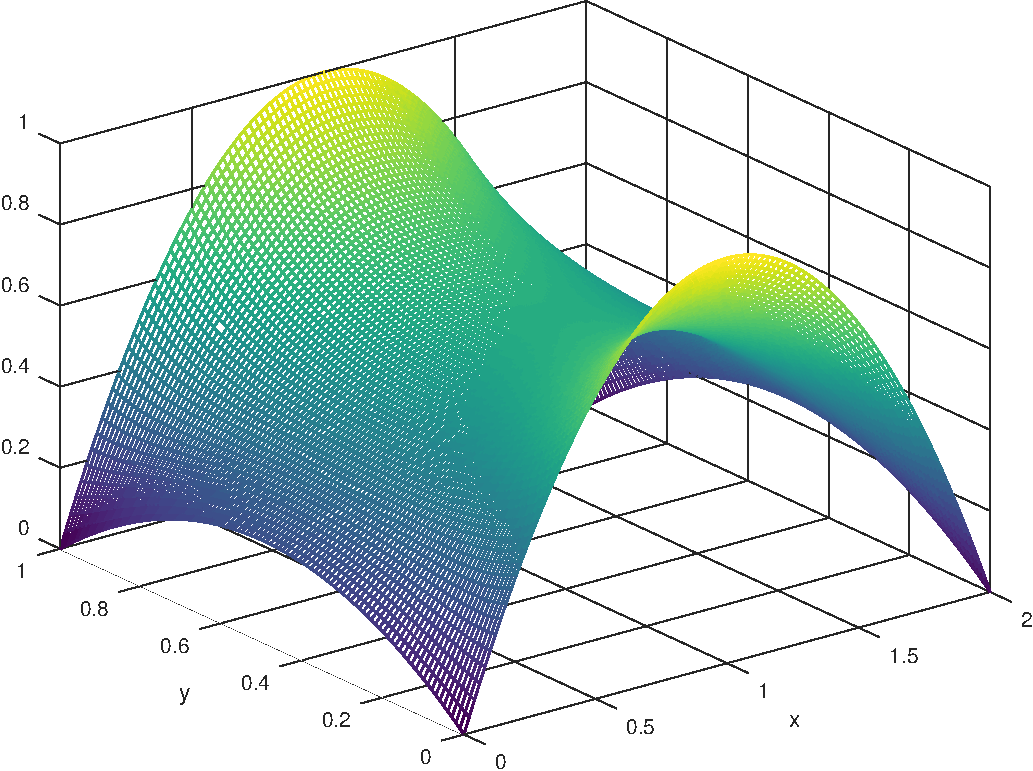
\includegraphics[width = \textwidth]{chapter_08/exercise_08_43_figure.pdf}
\end{center}


